\documentclass[tikz,convert={density=800,outext=.png},border=5pt]{standalone}
%\documentclass[tikz, border=5pt]{standalone}

\usepackage[utf8]{inputenc} % utf8 encoding
\usepackage[english]{babel}
\usepackage[T1]{fontenc} % use T1 fonts
\usepackage{amsmath} % nice math symbols
     

\usepackage{tikz}
\usetikzlibrary{shapes,positioning,calc,patterns,decorations.pathreplacing}

\newcommand{\situation}[3]{
	\node[draw, circle, fill=white, scale=1.5] (sit_#1) at (#2pt,#3pt) {};
}
\begin{document}
	
	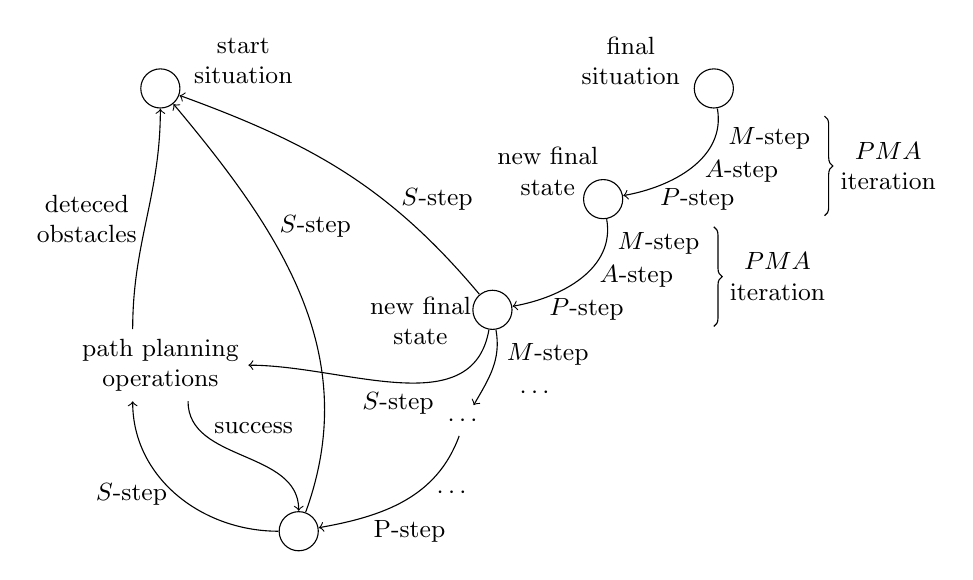
\begin{tikzpicture}[scale=2.0]
		\situation{st}{0}{0};
		\node[align=center, font=\small] at (15pt,5pt) {start\\situation};
		\situation{end}{100}{0};
		\node[align=center, font=\small] at (85pt,5pt) {final\\situation};
		
		
		\situation{1}{80}{-20};
		\situation{2}{60}{-40};
		\node[font=\small] (all) at (55pt,-60pt) {$\cdots$};
		\situation{3}{25}{-80};
		
		\draw[->] (sit_end) to[out=-80,in=10] (sit_1);
		\draw[->] (sit_1) to[out=-80,in=10] (sit_2);
		\draw[->] (all) to[out=-110,in=10] (sit_3);
		\draw[->] (sit_2) to[out=130,in=-20] (sit_st);
		\draw[->] (sit_2) to[out=-80,in=60] (all);
		
		\node[align=center, font=\small] at (110pt,-9pt) {$M$-step};
		\node[align=center, font=\small] at (105pt,-15pt) {$A$-step};
		\node[align=center, font=\small] at (97pt,-20pt) {$P$-step};
		\draw [decorate,decoration={brace,amplitude=3pt,mirror}]
		(120pt,-23pt) -- (120pt,-5pt) node[align=center,midway,font=\small,xshift=23pt] {$PMA$\\iteration};
		\node[align=center, font=\small] at (70pt,-15pt) {new final\\state};
		
		\node[align=center, font=\small] at (90pt,-28pt) {$M$-step};
		\node[align=center, font=\small] at (86pt,-34pt) {$A$-step};
		\node[align=center, font=\small] at (77pt,-40pt) {$P$-step};
		\draw [decorate,decoration={brace,amplitude=3pt,mirror}]
		(100pt,-43pt) -- (100pt,-25pt) node[align=center,midway,font=\small,xshift=23pt] {$PMA$\\iteration};		
		\node[align=center, font=\small] at (47pt,-42pt) {new final\\state};

		\node[align=center, font=\small] at (70pt,-48pt) {$M$-step};
		\node[align=center, font=\small] at (68pt,-55pt) {$\cdots$};

		\node[align=center, font=\small] at (53pt,-73pt) {$\cdots$};
		\node[align=center, font=\small] at (45pt,-80pt) {P-step};
		
		\node[align=center, font=\small] at (50pt,-20pt) {$S$-step};
		\node[align=center, font=\small] at (28pt,-25pt) {$S$-step};
		
		\node[align=center, font=\small] (ppo) at (0pt,-50pt) {path planning\\operations};
		\draw[->] (sit_3) to[out=-180, in = -90] node[font=\small,left]{$S$-step} ([xshift=-5pt]ppo.south);
		\draw[->] (sit_2) to[out=-100, in = 0] node[font=\small,below]{$S$-step} (ppo.east);
		\draw[->] ([xshift=5pt]ppo.south) to[out=-90, in = 90] node[font=\small,right,yshift=10pt,xshift=-14pt] {success} (sit_3);
		
		\draw[->] ([xshift=-5pt]ppo.north) to[out=90,in=-90] node[align=center,left, font=\small]{deteced\\obstacles} (sit_st);
		
		\draw[->] (sit_3) to[out=70, in = -50] (sit_st);
	\end{tikzpicture}


\end{document}